\documentclass[aspectratio=169]{beamer}
\usepackage{hyperref}
\usepackage{xcolor}
\usepackage{graphicx}
\usepackage{tikz}
\usetikzlibrary{positioning}
\usepackage{authoraftertitle}
\usepackage{fontspec}

\setsansfont{Oswald}[Path=./OswaldFontFiles/,Scale=0.9,Extension=.ttf,UprightFont=*-Regular,BoldFont=*-Bold]
    
\setromanfont{Lato}[Path=./LatoFontFiles/,Scale=0.9,Extension=.ttf,UprightFont=*-Regular,BoldFont=*-Bold]    

\setbeamertemplate{navigation symbols}{}
\setbeamertemplate{background}{\tikz[overlay, remember picture]%
  \node[anchor=south] at (current page.south)
     {
\includegraphics[width=.45\paperwidth]{img/slider-in}};}

\author{Dégi Nándor \\ Dr. Csató Lehel}
\title{Szimbólikus zenegenerálás gépi tanulással}
\newcommand\Facultate{Magyar Matematika és Informatika Intézet}
\newcommand\Universitate{Babe\c{s}-Bolyai tudományegyetem}
\newcommand\Adresa{Str. Mihail Kog\u{a}lniceanu nr. 1\\ Cluj-Napoca, Cluj, Rom\^{a}nia}
\newcommand\Website{www.cs.ubbcluj.ro}
\newcommand\DataPrezentarii{\today}

\usepackage{CSTheme_RO}

\begin{document}

%GENERARE PAGINA DE TITLU
%custom/title.tex
% Title slide frame
\begin{frame}[plain]
\begin{tikzpicture}[remember picture,overlay]
% Background image
\node[above right,inner sep=0pt] at (current page.south west)
{
    \includegraphics[width=\paperwidth]{img/blueCS_background.png}
};
    
% Title
\node[anchor=center, color=yellowCS, align=center, text width=14cm] (title) at ([yshift=0.5cm]current page.center)
{
    \Huge \MyTitle
};

% Separator Line
\draw[yellowCS, ultra thick] ([yshift=-0.5cm, xshift=-4cm]title.south) -- ([yshift=-0.5cm, xshift=4cm]title.south);

% Author 
\node[anchor=north, color=white, align=center] (author) at ([yshift=-1cm]title.south)
{
    \Large \MyAuthor
};

% Facultate
\node[anchor=north, color=yellowCS, align=center] (date1) at ([yshift=-0.8cm]author.south)
{
    \large \Facultate
};

% Universitate
\node[anchor=north, color=white, align=center] (date2) at ([yshift=-0.1cm]date1.south)
{
    \large \Universitate
};

% Logo CS
\node[anchor=north west] at ([xshift=1cm, yshift=-1cm]current page.north west)
{
    
\includegraphics[width=2cm]{img/CS_white_logo.png}
};

% Logo UBB
\node[anchor=north east] at ([xshift=-1cm, yshift=-1cm]current page.north east)
{
    
\includegraphics[width=2cm]{img/Sigla_UBB_claudiopolitana_alb.png}
};

\end{tikzpicture}
\end{frame}


%1. MIÉRT CSINÁLTAM EZT A PROJEKTET?
\begin{frame}{Miért csináltam ezt a projektet?}
\begin{itemize}
    \item \textbf{Személyes motiváció}: Zenélek, és mindig is szerettem volna saját zenekart
    \item \textbf{Kíváncsiság}: Vajon tudok-e valami jót alkotni mesterséges intelligenciával?
    \item \textbf{Kérdés}: Képesek-e a neurális hálózatok olyan zenét generálni, ami közel áll az emberi kreativitáshoz?
    \item \textbf{Cél}: Olyan rendszer kifejlesztése, amely segít zenei ötletek generálásában
\end{itemize}

\vspace{1em}
\begin{center}
\textit{„A zene és a matematika találkozása - lehet-e a gépi tanulás a kreativitás eszköze?"}
\end{center}
\end{frame}

%2. ÁTTEKINTÉS
\begin{frame}{Projekt áttekintés}
\begin{columns}[T]
\begin{column}{0.48\textwidth}
\textbf{Kutatási kérdések:}
\begin{itemize}
    \item Hogyan modellezhetjük a zenei struktúrákat?
    \item Hogyan őrizhetjük meg a zenei szimmetriákat?
    \item Hogyan generálhatunk új, értelmes zenét?
\end{itemize}
\end{column}

\begin{column}{0.48\textwidth}
\textbf{Implementált modellek:}
\begin{enumerate}
    \item Markov-láncok (baseline)
    \item Variációs Autoenkóder (VAE)
    \item \alert{GOLC-VAE (saját fejlesztés)}
    \item Transformer
\end{enumerate}
\end{column}
\end{columns}

\vspace{1em}
\begin{center}
\textbf{Adathalmaz}: MIDI fájlok gyűjteménye különböző zenei stílusokban
\end{center}
\end{frame}

%3. RENDSZER ARCHITEKTÚRA 
\begin{frame}{Rendszer architektúra}
\begin{center}
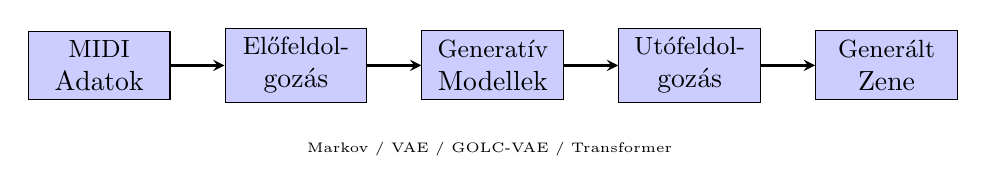
\begin{tikzpicture}[
    box/.style={rectangle, draw, fill=blue!20, minimum width=1.8cm, minimum height=0.8cm, align=center},
    arrow/.style={->, >=stealth, thick}
]
    \node[box] (data) at (0,0) {\small MIDI\\Adatok};
    \node[box] (preprocess) at (2.5,0) {\small Előfeldol-\\gozás};
    \node[box] (models) at (5,0) {\small Generatív\\Modellek};
    \node[box] (postprocess) at (7.5,0) {\small Utófeldol-\\gozás};
    \node[box] (output) at (10,0) {\small Generált\\Zene};
    
    \draw[arrow] (data) -- (preprocess);
    \draw[arrow] (preprocess) -- (models);
    \draw[arrow] (models) -- (postprocess);
    \draw[arrow] (postprocess) -- (output);
    
    \node[below=0.4cm of models, align=center, font=\tiny] {
        Markov / VAE / GOLC-VAE / Transformer
    };
\end{tikzpicture}
\end{center}

\vspace{0.5em}
\textbf{Technológiai stack:}
\begin{itemize}
    \item \textbf{Backend}: Python, PyTorch, FastAPI
    \item \textbf{Adatkezelés}: MIDI parsing, note encoding
    \item \textbf{Infrastruktúra}: Docker, GPU support
\end{itemize}
\end{frame}

%4. MARKOV LÁNCOK
\begin{frame}{Markov-láncok alapú generálás}
\begin{columns}[T]
\begin{column}{0.58\textwidth}
\textbf{Alapelv}: A következő állapot csak a jelenlegitől függ

\[
P(X_{t+1} = s_j \mid X_t = s_i) = p_{ij}
\]

\textbf{Példa}: Ha most C hangot hallunk, mi következik?
\begin{itemize}
    \item $P(\text{C} \to \text{D}) = 0.3$
    \item $P(\text{C} \to \text{E}) = 0.5$
    \item $P(\text{C} \to \text{G}) = 0.2$
\end{itemize}

\textbf{Implementáció}:
\begin{itemize}
    \item Magasabb rendű (2-6. rend)
    \item Hidden Markov Model (HMM)
    \item GPU gyorsítás, Sparse mátrix
\end{itemize}
\end{column}

\begin{column}{0.38\textwidth}
\vspace{0.5em}
\begin{center}
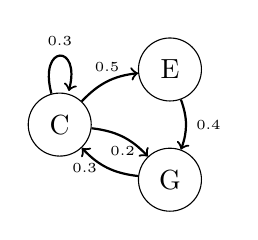
\begin{tikzpicture}[scale=0.7,
    node/.style={circle, draw, minimum size=0.8cm}]
    \node[node] (C) at (0,0) {C};
    \node[node] (E) at (2,1) {E};
    \node[node] (G) at (2,-1) {G};
    
    \draw[->, thick, bend left=20] (C) to node[above,font=\tiny] {0.5} (E);
    \draw[->, thick, bend left=20] (C) to node[below,font=\tiny] {0.2} (G);
    \draw[->, thick, bend left=20] (E) to node[right,font=\tiny] {0.4} (G);
    \draw[->, thick, bend left=20] (G) to node[left,font=\tiny] {0.3} (C);
    \draw[->, thick] (C) edge [loop above] node[above,font=\tiny] {0.3} (C);
\end{tikzpicture}
\end{center}

\vspace{0.5em}
\textbf{Előnyök/hátrányok:}
\begin{itemize}
    \item[\textcolor{green}{+}] Gyors, értelmezhető
    \item[\textcolor{red}{-}] Csak lokális struktúra
    \item[\textcolor{red}{-}] Nincs globális koherencia
\end{itemize}
\end{column}
\end{columns}
\end{frame}

%5. VAE ALAPOK
\begin{frame}{Variációs Autoenkóder (VAE)}
\textbf{Cél}: Kompresszálja a zenét egy kompakt reprezentációba, majd visszafejti

\begin{center}
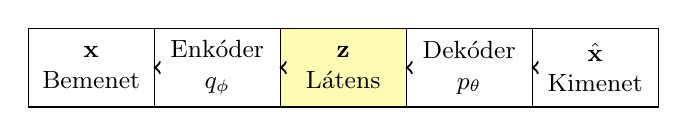
\begin{tikzpicture}[
    node distance=1.6cm,
    box/.style={rectangle, draw, minimum width=1.6cm, minimum height=1cm, align=center, font=\small}
]
    \node[box] (input) {$\mathbf{x}$\\Bemenet};
    \node[box, right of=input] (encoder) {Enkóder\\$q_\phi$};
    \node[box, right of=encoder, fill=yellow!30] (latent) {$\mathbf{z}$\\Látens};
    \node[box, right of=latent] (decoder) {Dekóder\\$p_\theta$};
    \node[box, right of=decoder] (output) {$\hat{\mathbf{x}}$\\Kimenet};
    
    \draw[->, thick] (input) -- (encoder);
    \draw[->, thick] (encoder) -- (latent);
    \draw[->, thick] (latent) -- (decoder);
    \draw[->, thick] (decoder) -- (output);
\end{tikzpicture}
\end{center}

\vspace{0.3em}
\textbf{Reparametrizációs trükk} (hogy gradiens visszaáramolhasson):
\begin{center}
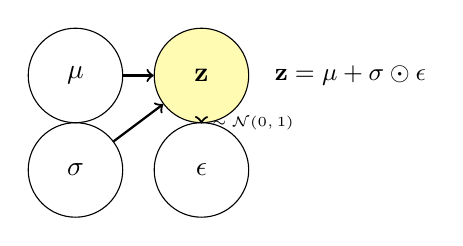
\begin{tikzpicture}[scale=0.8]
    \node[draw, circle, minimum size=1.2cm] (mu) at (0,0) {$\boldsymbol{\mu}$};
    \node[draw, circle, minimum size=1.2cm] (sigma) at (0,-1.5) {$\boldsymbol{\sigma}$};
    \node[draw, circle, minimum size=1.2cm] (eps) at (2,-1.5) {$\boldsymbol{\epsilon}$};
    \node[draw, circle, minimum size=1.2cm, fill=yellow!30] (z) at (2,0) {$\mathbf{z}$};
    
    \draw[->, thick] (mu) -- (z);
    \draw[->, thick] (sigma) -- (z);
    \draw[->, thick] (eps) -- (z) node[midway, right, font=\tiny] {$\sim \mathcal{N}(0,1)$};
    
    \node[right=0.2cm of z, font=\small] {$\mathbf{z} = \boldsymbol{\mu} + \boldsymbol{\sigma} \odot \boldsymbol{\epsilon}$};
\end{tikzpicture}
\end{center}

\vspace{0.3em}
\textbf{Veszteségfüggvény}:
\[
\mathcal{L} = \underbrace{\|\mathbf{x} - \hat{\mathbf{x}}\|^2}_{\text{Rekonstrukció}} + \beta \cdot \underbrace{D_{\text{KL}}(q_\phi \parallel p)}_{\text{Regularizáció}}
\]
\end{frame}

%6. GOLC-VAE SLIDE 1 - A PROBLÉMA
\begin{frame}{A probléma: Transzpozíciós invariancia}
\textbf{Megfigyelés}: Egy dallam transzponálva is ugyanaz marad zeneileg

\vspace{0.5em}
\begin{columns}[T]
\begin{column}{0.55\textwidth}
\textbf{Probléma a standard VAE-vel}:
\begin{itemize}
    \item Ugyanazt a dallamot különböző hangnemekben külön reprezentációként tanulja
    \item Felesleges redundancia a látens térben
    \item Nem használja ki a zenei szimmetriákat
\end{itemize}

\vspace{0.5em}
\alert{Megoldás: Csoport-Orbitális Látens Konzisztencia (GOLC)}
\end{column}

\begin{column}{0.42\textwidth}
\vspace{-0.5em}
\begin{center}
\textbf{Példa:}\\
\vspace{0.3em}
\textit{C-E-G} (C-dúr hármas)\\
\textit{D-F\#-A} (D-dúr hármas)\\
\textit{E-G\#-B} (E-dúr hármas)

\vspace{0.5em}
\tikz{
    \node[draw, circle, fill=red!30] at (0,0) {z₁};
    \node[draw, circle, fill=red!30] at (1,0.5) {z₂};
    \node[draw, circle, fill=red!30] at (0.5,-0.5) {z₃};
}

\vspace{0.3em}
Standard VAE:\\3 különböző pont

\vspace{0.5em}
\tikz{
    \node[draw, circle, fill=green!40] at (0.5,0) {z};
}

\vspace{0.3em}
GOLC-VAE:\\1 közös pont
\end{center}
\end{column}
\end{columns}
\end{frame}

%7. GOLC-VAE SLIDE 2 - A MEGOLDÁS
\begin{frame}{GOLC-VAE: Saját innovációm}
\textbf{Alapötlet}: Explicit módon beépítjük a zenei szimmetriákat

\vspace{0.5em}
\textbf{Kulcs fogalmak}:
\begin{itemize}
    \item \textbf{Orbit}: Egy dallam összes transzponált változata
    \item \textbf{Kanonikus reprezentáció}: Az orbit átlaga a látens térben
    \item \textbf{Orbitális konzisztencia}: $\text{Enc}(g \cdot \mathbf{x}) \approx \text{Enc}(\mathbf{x})$ minden $g \in G$-re
\end{itemize}

\vspace{0.5em}
\textbf{Bővített veszteségfüggvény}:
\[
\mathcal{L}_{\text{total}} = \mathcal{L}_{\text{recon}} + \beta \cdot \mathcal{L}_{\text{KL}} + \alert{\beta_{\text{orbit}} \cdot \mathcal{L}_{\text{orbit}}}
\]

\vspace{0.5em}
ahol:
\[
\mathcal{L}_{\text{orbit}} = \frac{1}{|G|} \sum_{g \in G} \|\mu(\mathbf{x}) - \mu(g \cdot \mathbf{x})\|^2
\]
\end{frame}

%8. GOLC-VAE IMPLEMENTÁCIÓ
\begin{frame}{GOLC-VAE: Implementáció}
\textbf{Orbitális konzisztencia számítása (pszeudokód):}

\begin{center}
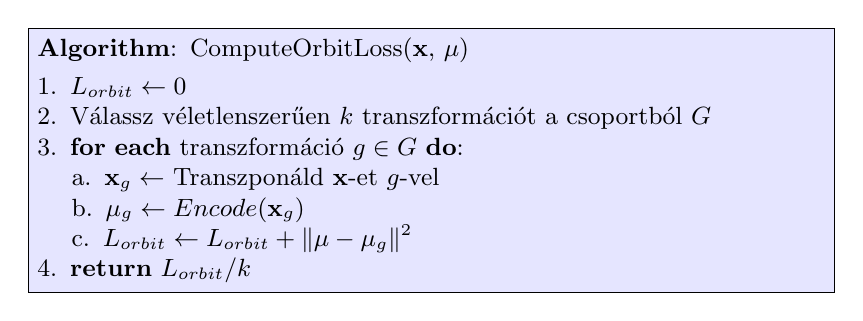
\begin{tikzpicture}[node distance=0.2cm]
\node[draw, rectangle, fill=blue!10, text width=10cm, font=\small, align=left] (algo) {
\textbf{Algorithm}: ComputeOrbitLoss($\mathbf{x}$, $\boldsymbol{\mu}$)\\[0.3em]
1. $L_{\text{orbit}} \gets 0$\\
2. Válassz véletlenszerűen $k$ transzformációt a csoportból $G$\\
3. \textbf{for each} transzformáció $g \in G$ \textbf{do}:\\
\hspace{1em} a. $\mathbf{x}_g \gets$ Transzponáld $\mathbf{x}$-et $g$-vel\\
\hspace{1em} b. $\boldsymbol{\mu}_g \gets \text{Encode}(\mathbf{x}_g)$\\
\hspace{1em} c. $L_{\text{orbit}} \gets L_{\text{orbit}} + \|\boldsymbol{\mu} - \boldsymbol{\mu}_g\|^2$\\
4. \textbf{return} $L_{\text{orbit}} / k$
};
\end{tikzpicture}
\end{center}

\vspace{0.5em}
\textbf{Lényeg}: Minden transzponált változat ugyanarra a látens pontra képződjön

\vspace{0.3em}
\textbf{Optimalizáció}: Nem minden transzformációt számolunk ki, csak mintavételezünk
\end{frame}

%9. TRANSFORMER MODELL
\begin{frame}{Transformer modell zenei generáláshoz}
\begin{columns}[T]
\begin{column}{0.55\textwidth}
\textbf{Mi a Transformer?}
\begin{itemize}
    \item Eredeti cél: Szövegfordítás (GPT, BERT alapja)
    \item \textbf{Self-attention}: Minden hang "figyel" minden más hangra
    \item \textbf{Pozíciókódolás}: Megjegyzi a hangok sorrendjét
\end{itemize}

\vspace{0.5em}
\textbf{Zenei alkalmazás}:
\begin{itemize}
    \item Hosszú távú függőségek (pl. visszatérő témák)
    \item Harmonikus struktúra (akkordok közti viszonyok)
    \item Ritmus mintázatok felismerése
\end{itemize}

\vspace{0.5em}
\textbf{Előnyök/hátrányok}:
\begin{itemize}
    \item[\textcolor{green}{+}] Globális kontextus
    \item[\textcolor{green}{+}] Párhuzamosítható
    \item[\textcolor{red}{-}] Nagy memóriaigény
\end{itemize}
\end{column}

\begin{column}{0.42\textwidth}
\vspace{0.5em}
\begin{center}
\textbf{Attention mechanizmus:}
\vspace{0.3em}

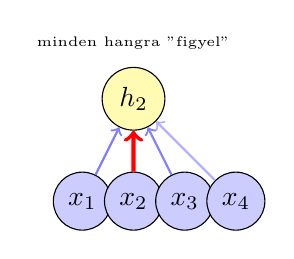
\begin{tikzpicture}[scale=0.65]
    % Input notes
    \node[draw, circle, fill=blue!20] (n1) at (0,0) {$x_1$};
    \node[draw, circle, fill=blue!20] (n2) at (1,0) {$x_2$};
    \node[draw, circle, fill=blue!20] (n3) at (2,0) {$x_3$};
    \node[draw, circle, fill=blue!20] (n4) at (3,0) {$x_4$};
    
    % Attention
    \node[draw, circle, fill=yellow!30] (a2) at (1,2) {$h_2$};
    
    % Arrows showing attention
    \draw[->, thick, blue!50] (n1) -- (a2);
    \draw[->, thick, red, line width=1.5pt] (n2) -- (a2);
    \draw[->, thick, blue!50] (n3) -- (a2);
    \draw[->, thick, blue!30] (n4) -- (a2);
    
    \node[above=0.1cm of a2, font=\tiny] {minden hangra "figyel"};
\end{tikzpicture}

\vspace{0.5em}
\small
$\text{Attention}(Q,K,V) = \text{softmax}\left(\frac{QK^T}{\sqrt{d_k}}\right)V$

\vspace{0.5em}
\textit{A piros nyíl mutatja, hogy $x_2$ magára figyel a legjobban}
\end{center}
\end{column}
\end{columns}
\end{frame}

%10. EREDMÉNYEK 1
\begin{frame}{Eredmények: Összehasonlítás}
\textbf{Értékelési metrikák}:
\begin{itemize}
    \item \textbf{Rekonstrukciós hiba}: Mennyire jól rekonstruálja az eredeti zenét
    \item \textbf{Pitch distribution}: A hangmagasságok eloszlása
    \item \textbf{Orbitális konzisztencia}: Transzpozíciós invariancia mértéke
\end{itemize}

\vspace{0.5em}
\begin{table}[h]
\centering
\footnotesize
\begin{tabular}{|l|c|c|c|}
\hline
\textbf{Modell} & \textbf{Recon. Loss} & \textbf{Orbit Cons.} & \textbf{Minőség} \\
\hline
Markov & - & - & Közepes \\
Baseline VAE & 0.082 & 2.34 & Jó \\
\alert{GOLC-VAE} & \alert{0.078} & \alert{0.45} & \alert{Nagyon jó} \\
Transformer & 0.075 & - & Nagyon jó \\
\hline
\end{tabular}
\end{table}

\vspace{0.5em}
\alert{GOLC-VAE: 5.2× jobb orbitális konzisztencia!}
\end{frame}

%11. EREDMÉNYEK 2
\begin{frame}{Eredmények: GOLC-VAE hatása}
\textbf{Fő megállapítások}:

\begin{enumerate}
    \item \textbf{Transzpozíciós invariancia}: A GOLC-VAE sikeresen megtanulja, hogy különböző hangnemek ugyanazt a zenei tartalmat képviselik
    
    \item \textbf{Látens tér struktúra}: Az orbit-átlagolás kompaktabb, értelmesebb látens teret eredményez
    
    \item \textbf{Generálási minőség}: A zenei szimmetriák beépítése javítja a generált zene koherenciáját
    
    \item \textbf{Általánosítás}: A modell jobban általánosít új, látott stílusokra
\end{enumerate}

\vspace{0.5em}
\begin{center}
\textit{A zenei strukturális tulajdonságok beépítése kulcsfontosságú a jobb generáláshoz}
\end{center}
\end{frame}

%12. TECHNIKAI KIHÍVÁSOK
\begin{frame}{Technikai kihívások és megoldások}
\begin{itemize}
    \item \textbf{Kihívás 1}: MIDI adatok előfeldolgozása
    \begin{itemize}
        \item Megoldás: Egységes note encoding, normalizáció
    \end{itemize}
    
    \item \textbf{Kihívás 2}: GPU memória kezelés nagyobb modellekkel
    \begin{itemize}
        \item Megoldás: Gradient checkpointing, batch size optimalizálás
    \end{itemize}
    
    \item \textbf{Kihívás 3}: Orbitális veszteség számítási költsége
    \begin{itemize}
        \item Megoldás: Mintavételezés a transzformációs csoportból
    \end{itemize}
    
    \item \textbf{Kihívás 4}: Kiegyensúlyozás a különböző veszteség tagok között
    \begin{itemize}
        \item Megoldás: Hiperparaméter tuning ($\beta$, $\beta_{\text{orbit}}$)
    \end{itemize}
\end{itemize}
\end{frame}

%13. DEMO ÉS ALKALMAZÁS
\begin{frame}{Gyakorlati alkalmazás}
\textbf{FastAPI backend}:
\begin{itemize}
    \item REST API a generáláshoz
    \item Kreativitás paraméter (0-1): szabályozza a véletlenszerűséget
    \item Időtartam és hangszer beállítás
    \item MIDI fájl kimenet
\end{itemize}

\vspace{0.5em}
\textbf{Felhasználási módok}:
\begin{enumerate}
    \item \textbf{Inspiráció}: Teljesen új zenei ötletek generálása
    \item \textbf{Variációk}: Meglévő dallamok variálása és továbbfejlesztése
    \item \textbf{Kiegészítés}: Részleges kompozíciók befejezése
    \item \textbf{Stílustanulás}: Különböző zenei stílusok (Bach, Jazz, stb.) modellezése
\end{enumerate}

\vspace{0.5em}
\begin{center}
\textit{A rendszer támogatja az interaktív munkamódot is}
\end{center}
\end{frame}

%14. KONKLÚZIÓ
\begin{frame}{Konklúzió és jövőbeli munka}
\textbf{Elért eredmények}:
\begin{itemize}
    \item[\checkmark] Több generatív modell összehasonlító implementációja
    \item[\checkmark] \alert{GOLC-VAE}: Új módszer a zenei szimmetriák beépítésére
    \item[\checkmark] Jelentős javulás az orbitális konzisztenciában (5.2×)
    \item[\checkmark] Működő rendszer zenei generálásra
\end{itemize}

\vspace{0.5em}
\textbf{Jövőbeli irányok}:
\begin{itemize}
    \item További zenei szimmetriák beépítése (ritmus, harmónia)
    \item Több hangszer egyidejű generálása
    \item Valós idejű interaktív generálás
    \item Felhasználói feedback beépítése (reinforcement learning)
\end{itemize}

\vspace{0.5em}
\begin{center}
\textit{„A gépi tanulás nem helyettesíti az emberi kreativitást, hanem kiegészíti azt"}
\end{center}
\end{frame}

%15. KÖSZÖNETNYILVÁNÍTÁS
\begin{frame}{}
\begin{center}
{\Large Köszönöm a figyelmet!}

\vspace{2em}

\textbf{Köszönet}:
\begin{itemize}
    \item Dr. Csató Lehel témavezetőmnek a szakmai irányításért
    \item A Babeș-Bolyai Tudományegyetem Matematika és Informatika Karának
    \item Családomnak és barátaimnak a támogatásért
\end{itemize}

\vspace{2em}

{\large Kérdések?}

\vspace{1em}

\footnotesize
\textbf{Projekt}: \url{https://github.com/Dedzsinator/Zha}\\
\textbf{Email}: degi.nandor@example.com
\end{center}
\end{frame}

\end{document}
